% Options for packages loaded elsewhere
\PassOptionsToPackage{unicode}{hyperref}
\PassOptionsToPackage{hyphens}{url}
%
\documentclass[
  ignorenonframetext,
]{beamer}
\usepackage{pgfpages}
\setbeamertemplate{caption}[numbered]
\setbeamertemplate{caption label separator}{: }
\setbeamercolor{caption name}{fg=normal text.fg}
\beamertemplatenavigationsymbolsempty
% Prevent slide breaks in the middle of a paragraph
\widowpenalties 1 10000
\raggedbottom
\setbeamertemplate{part page}{
  \centering
  \begin{beamercolorbox}[sep=16pt,center]{part title}
    \usebeamerfont{part title}\insertpart\par
  \end{beamercolorbox}
}
\setbeamertemplate{section page}{
  \centering
  \begin{beamercolorbox}[sep=12pt,center]{part title}
    \usebeamerfont{section title}\insertsection\par
  \end{beamercolorbox}
}
\setbeamertemplate{subsection page}{
  \centering
  \begin{beamercolorbox}[sep=8pt,center]{part title}
    \usebeamerfont{subsection title}\insertsubsection\par
  \end{beamercolorbox}
}
\AtBeginPart{
  \frame{\partpage}
}
\AtBeginSection{
  \ifbibliography
  \else
    \frame{\sectionpage}
  \fi
}
\AtBeginSubsection{
  \frame{\subsectionpage}
}
\usepackage{lmodern}
\usepackage{amssymb,amsmath}
\usepackage{ifxetex,ifluatex}
\ifnum 0\ifxetex 1\fi\ifluatex 1\fi=0 % if pdftex
  \usepackage[T1]{fontenc}
  \usepackage[utf8]{inputenc}
  \usepackage{textcomp} % provide euro and other symbols
\else % if luatex or xetex
  \usepackage{unicode-math}
  \defaultfontfeatures{Scale=MatchLowercase}
  \defaultfontfeatures[\rmfamily]{Ligatures=TeX,Scale=1}
\fi
\usetheme[]{CambridgeUS}
% Use upquote if available, for straight quotes in verbatim environments
\IfFileExists{upquote.sty}{\usepackage{upquote}}{}
\IfFileExists{microtype.sty}{% use microtype if available
  \usepackage[]{microtype}
  \UseMicrotypeSet[protrusion]{basicmath} % disable protrusion for tt fonts
}{}
\makeatletter
\@ifundefined{KOMAClassName}{% if non-KOMA class
  \IfFileExists{parskip.sty}{%
    \usepackage{parskip}
  }{% else
    \setlength{\parindent}{0pt}
    \setlength{\parskip}{6pt plus 2pt minus 1pt}}
}{% if KOMA class
  \KOMAoptions{parskip=half}}
\makeatother
\usepackage{xcolor}
\IfFileExists{xurl.sty}{\usepackage{xurl}}{} % add URL line breaks if available
\IfFileExists{bookmark.sty}{\usepackage{bookmark}}{\usepackage{hyperref}}
\hypersetup{
  pdftitle={Optimizing the Aquisition of Heavy Equiptment for Small Businesses},
  pdfauthor={David Hill, Jr.},
  hidelinks,
  pdfcreator={LaTeX via pandoc}}
\urlstyle{same} % disable monospaced font for URLs
\newif\ifbibliography
\usepackage{graphicx}
\makeatletter
\def\maxwidth{\ifdim\Gin@nat@width>\linewidth\linewidth\else\Gin@nat@width\fi}
\def\maxheight{\ifdim\Gin@nat@height>\textheight\textheight\else\Gin@nat@height\fi}
\makeatother
% Scale images if necessary, so that they will not overflow the page
% margins by default, and it is still possible to overwrite the defaults
% using explicit options in \includegraphics[width, height, ...]{}
\setkeys{Gin}{width=\maxwidth,height=\maxheight,keepaspectratio}
% Set default figure placement to htbp
\makeatletter
\def\fps@figure{htbp}
\makeatother
\setlength{\emergencystretch}{3em} % prevent overfull lines
\providecommand{\tightlist}{%
  \setlength{\itemsep}{0pt}\setlength{\parskip}{0pt}}
\setcounter{secnumdepth}{-\maxdimen} % remove section numbering

\title{Optimizing the Aquisition of Heavy Equiptment for Small
Businesses}
\author{David Hill, Jr.}
\date{April 2020}

\begin{document}
\frame{\titlepage}

\begin{frame}{Introduction}
\protect\hypertarget{introduction}{}
\begin{itemize}
\item
  With this project will introduce a decision analysis tool to help real
  estate development companies evaluate decisions for the acquisition of
  real-estate development equiptment.
\item
  The target decision maker for this tool is the owner or executive of a
  small-medium sized real-estate development company.
\item
  For companies of this nature, financial resources are often limited so
  it is imperitive for them to make a wise decision regarding the
  acquisition of heavy equiptment.
\item
  The goal of this project is to augment a classic rent vs buy analysis
  with a catastrophic failure analysis of equiptment based on use.
\end{itemize}
\end{frame}

\begin{frame}{Motivation}
\protect\hypertarget{motivation}{}
\begin{itemize}
\item
  A poor acquisition decision can lead to project failure, injury to
  personnel and significant loss of capital which can be crippling to a
  small business.
\item
  Making the right acquisition decisons can greatly improve the
  financial posture of the business by reducing cost and risk.
\item
  Inform decision makers as to which method of acquisition makes sense
  for their business and what condition of equiptment they should
  acquire to meet their goals.
\end{itemize}
\end{frame}

\begin{frame}{Decision Problem}
\protect\hypertarget{decision-problem}{}
\begin{itemize}
\tightlist
\item
  The main decision the business owner must make is whether they should
  buy or lease the equiptment, should they buy with a loan or in cash,
  and what condition of equiptment should they buy (new, used, or very
  used).
\end{itemize}
\end{frame}

\begin{frame}{Decision Problem Cont'd}
\protect\hypertarget{decision-problem-contd}{}
We define the decision maker's action set \(\ A\) as the set of actions
the user can make within our decision tool.
\end{frame}

\begin{frame}{Decision Problem: Action Set}
\protect\hypertarget{decision-problem-action-set}{}
Let \(\alpha_{1}\), \(\alpha_{2}\) ,\ldots, \(\alpha_{n} \in \ A\)

where:

\(\alpha_{1}\) = Buy a new bulldozer with cash

\(\alpha_{3}\) = Buy a new bulldozer with loan

\(\alpha_{5}\) = Rent a bulldozer

\(\alpha_{6}\) = Buy a used bulldozer with cash

\(\alpha_{6}\) = Buy a used bulldozer with loan
\end{frame}

\begin{frame}{Decision Problem: State Space}
\protect\hypertarget{decision-problem-state-space}{}
We define the state space \(\ X\) as the set of possible outcomes.

Let \(\chi_{1}, \chi_{2} \in \ X\)

where:

\(\chi_{1}\) = 1, The bulldozer suffers a catastrophic failure

\(\chi_{2}\) = 0, The bulldozer does not suffer a catastrophic failure.

We assume our random variable will take the form of a Poisson
distribution over a period of time.
\end{frame}

\begin{frame}{Decision Problem: Parameter Space}
\protect\hypertarget{decision-problem-parameter-space}{}
We define the parameter space \(\Theta\) as the set of unobserved
parameters that will represent the period of time until a catastrophic
failure is expected.

Let \(\theta_{1}\), \(\theta_{2}\) ,\ldots, \(\theta_{n} \in \Theta\)

where:

\(\theta_{1}\) = The probability of a catastrophic mechanical failure in
the next 5 years

\(\theta_{2}\) = The probability of a catastrophic mechanical failure in
the next 10 years

\(\theta_{3}\) = The probability of a catastrophic mechanical failure in
the next 15 years
\end{frame}

\begin{frame}{Poisson Distribution}
\protect\hypertarget{poisson-distribution}{}
Expresses the probability of a given number of events occurring in a
fixed interval of time or space if these events occur with a known
constant mean rate and independently of the time since the last event.

A discrete random variable \(\chi\) is said to have a Poisson
distribution with parameter \(\lambda\) \textgreater{} 0, if, for
\(\chi\) = 0, 1, 2, \ldots, the probability mass function of \(\chi\) is
given by:

\(P(\chi = \ X) = \frac{\lambda^{\chi} \times e^{-\lambda}}{\chi !}\)

where:

\(\mu = \lambda\)

\(\sigma^{2} = \lambda\)

\(e = 2.71828...\)
\end{frame}

\begin{frame}{Data}
\protect\hypertarget{data}{}
\begin{itemize}
\item
  Difficult to find bulldozer failure data
\item
  Generate data sets using python based on used bulldozer sellers
\item
  Bulldozer price is mainly based on work hours, age plays a small
  factor
\item
  Data set represents bulldozers that filed in a year
\item
  With this data set we can calculate the failure rate and lambda values
  for our poisson function
\end{itemize}
\end{frame}

\begin{frame}{Data: Cont'd}
\protect\hypertarget{data-contd}{}
\begin{figure}
\centering
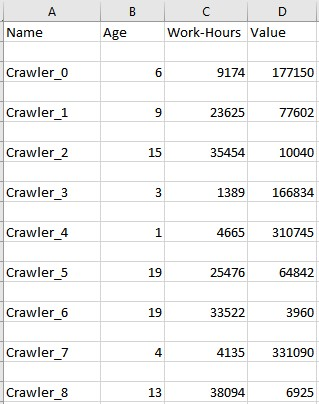
\includegraphics{./tex2pdf.-3403081cc63b4f47/7032243e87b12bb94f9ce8e7cf0561b5143a28d8.jpg}
\caption{Generated dataset}
\end{figure}
\end{frame}

\begin{frame}{Decision Problem: Example}
\protect\hypertarget{decision-problem-example}{}
According to collected bulldozer failure data, the average failure rate
for a bulldozer with 50,000 work hours is 0.7 catastrophic failures per
year. Failures follow a Poisson distribution. What is the probability
that this bulldozer will experience a catastrophic failure in the next 5
years?

\(\chi\) = number of failures expected = 1

\(\lambda = .7 * 5 = 3.5\)

\(P(\chi = 1) = \frac{\lambda^{\chi} \times e^{-\lambda}}{\chi !} = \frac{3.5^{1} \times e^{-3.5}}{1!} = 0.10569\)

Thus, within a 5 year period, a bulldozer with 50,000 work hours has a
10.6\% chance of experiencing a catastrophic failure.
\end{frame}

\begin{frame}{Predictive Model}
\protect\hypertarget{predictive-model}{}
\begin{itemize}
\item
  The novel predictive value this tool will provide is it's ability to
  predict catastrophic equiptment failure given it's wear. This will
  reduce uncertainty for a decision maker who is assessing used
  equiptment options.
\item
  This uncertainty is directly related to the payoff of our decision
  model as there is a monetary benefit to purchasing a used piece of
  equiptment over new equiptment. However, used equiptment poses a
  higher risk of catastrophic mechanical failure.
\end{itemize}
\end{frame}

\begin{frame}{Value}
\protect\hypertarget{value}{}
\begin{itemize}
\item
  The value of this tool is in minimizing the cost of ownership for the
  decision maker. The tool helps decion makers weigh the pros and cons
  of renting, buying new, and buying used and helps balance risk v.s
  monetary benefit to accomplish the organization's goals.
\item
  \(Payoff_{risk} = P(\chi = 1) * TotalCost\)
\item
  The lower the number the better as we want to minimize risk.
\end{itemize}
\end{frame}

\begin{frame}{The End}
\protect\hypertarget{the-end}{}
\end{frame}

\end{document}
